%!TEX root = ../book.tex
\chapter{Forces}\label{ch:forces}
%alessandro

So far, we have only been concerned with how robots move and the \textsl{geometry of motion}.
However, moving a robot not only requires a kinematic model of the platform under consideration, but also an understanding of the (generalized) forces needed to actuate the robot's motors and those needed for the robot to interact with the environment.
While this aspect can be ignored in basic applications of mobile robots and simple manipulation, it becomes critical as soon as robots interact more closely with people or need to engage in more complex manipulation: in these scenarios, \textsl{safety} and \textsl{model accuracy} are of paramount importance.

%The (geometric) Jacobian represents a fundamental tool to characterize the motion and the interaction of a robot with its environment, as it is used to perform the following \cite{sciavicco2012modelling}):
%\begin{enumerate}
%\item inverse differential kinematics even for robots that do not have a closed-form solution (\cref{sec:invjac});
%\item singularity analysis (a kinematic singularity is a robot configuration in which the robot loses the ability to move to one or more directions);
%\item redundancy analysis (a kinematic task is redundant if the robot possesses more degrees of freedom than what are needed to perform the task, resulting in infinite inverse kinematics solutions to choose from);
%\item manipulability analysis (i.e. how easy or difficult is it for a robot to move in a certain direction).
%\end{enumerate}
In this Chapter, we will introduce the reader to these concepts through \textsl{statics}\index{Statics}, which introduces a third abstraction to the problem of analyzing how robots move in space and interact with their surroundings.
More specifically, in \cref{sec:kinematics:fwd,sec:kinematics:ik} we have investigated the \textsl{kinematic} problem and operated in the space of \textsl{positions}, that is, how to map joint angles with end effector poses.
In \cref{sec:kinematics:diff}, we introduced the \textsl{differential kinematics} problem and operated in the space of \textsl{velocities}, i.e. how to map joint velocities with end-effector velocity twists (remember: velocity is derivative of position, hence the name ``differential'').
In the following, we will operate in the space of \textsl{forces}; however, we will simplify the more general dynamical problem by looking at the robot in static equilibrium---otherwise known as a \textsl{static} configuration.
As we will see, a lot can be done by simply looking at the robot in an equilibrium configuration!
The fourth and last abstraction, which goes beyond the scope of this book, is called \textsl{dynamics} and operates in the space of forces from a non-static perspective; it involves the second derivative of position (i.e. the acceleration), and it can be thought as a generalization of the second law of Newton ($F=ma$).
We will briefly introduce the reader to the topic in \cref{sec:forces:dynamics}.\td{remember to remove this sentence if we decide not to have the subchapter on dynamics}
%
The goals of this chapter are to:

\begin{itemize}
\item introduce the concept of statics
\item understand the so called ``kineto-statics duality''
\item become familiar with the notion of ``manipulability''
\item briefly introduce the dynamics problem.
\end{itemize}

Most of the concepts below are typically considered in the context of manipulation, as mobile robots generally do not exchange forces with their environment.
Therefore, for simplicity we will hereinafter refer to robot manipulators equipped with revolute joints unless otherwise specified.

\begin{mdframed}
\noindent The analysis of motion of a robot can be thought as a layered system with multiple levels of abstraction of increasing complexity.
The more complex it becomes, the more comprehensive your analysis will be, and the more capability you will be able to squeeze out of the robot!
However, it is good practice to start with the simplest layer first (i.e. kinematics), and gradually progress toward a dynamic analysis only if needed.
\end{mdframed}

\section{Statics}\label{sec:forces:statics}

\textsl{Statics} deals with relating (generalized) forces at the robot's joints and generalized forces at the end-effector when the robot is in \textsl{static equilibrium}, i.e. the acceleration of the robot and all of its components is zero.
If such a condition is met, a robot with $n$ degrees of freedom and an end-effector characterized by $m$ degrees of freedom can be fully described by the following quantities:
\begin{itemize}
    \item an $\left( n \times 1 \right)$ vector of generalized forces $\tau$ at the joints;
    \item an $\left( m \times 1 \right)$ vector of generalized forces $F$ exerted \textsl{by the robot end-effector} on the environment---or, more generally, by any part of the robot that may be in direct physical contact with the environment;
    \item an $\left( m \times 1 \right)$ vector of forces exerted \textsl{by the environment} on the robot end-effector $F_e$---which, per the principle of action and reaction, are equal and opposite to $F$: $F_e=-F$.
\end{itemize}
In this case, \textsl{generalized force}\index{Generalized Force} means ``any force-equivalent quantity needed to describe the element''.
In the case of joints, it depends on the actuation: generalized forces at the joints are either forces for prismatic joints (as they impart a translational motion on the joint) or torques for revolute joints (as they impart a rotational motion on the joint); the size of this vector depends on the number of mechanical degrees-of-freedom $n$.
In the case of the end-effector, it depends on the number of DoFs in task space $m$; if we are operating with a $6-$DoF problem, the $m \times 1$ vector of generalized forces will be composed of a linear force component given by the forces on the three axes:
\begin{equation}
f=\left[\begin{array}{c}
f_x\\
f_y\\
f_z
\end{array}
\right],
\end{equation}
and an angular force component (or moment) $\mu$ around the three axes:
\begin{equation}
\mu=\left[\begin{array}{c}
\mu_x\\
\mu_y\\
\mu_z
\end{array}
\right].
\end{equation}
We can now combine the above elements in a $6\times1$ vector as $F=[f \ \mu]^T$.
This vector of generalized forces is also called a \textsl{spatial force} or \textsl{wrench}\index{Wrench}\index{Spatial Force}.
We now want to compute the statics version of \cref{eq:kinematics:diff:fwd:short,eq:kinematics:diff:fwd}, and relate our $n \times 1$ vector of torques $\tau$ with the $6\times1$ wrench vector $F$.
To find this relationship, let's recall the definition of \textsl{power} from physics. Mechanical power $W$ is defined as force times velocity, which can be generalized as generalized forces times generalized velocities: $W=F^T \cdot \nu$.
Now, we know that the forces exchanged at the end-effector come from our source of actuation, i.e. our motors, whose generated power is defined by $W=\tau ^T \cdot \dot{q}$. We therefore have that:
\begin{equation}\label{eq:forces:statics:work}
W=\tau ^T \cdot \dot{q} = F^T  \cdot \nu
\end{equation}
We also know the relation between $\nu$ and $\dot{q}$ from \cref{eq:kinematics:diff:fwd:short}: $\nu =J(q) \cdot \dot{q}$. \cref{eq:forces:statics:work} then becomes:
\begin{equation}
\tau ^T \cdot \dot{q} = F^T  \cdot J(q) \cdot \dot{q} \ ,
\end{equation}
which, with minor rearrangements, turns into the following:
\begin{equation}\label{eq:forces:statics}
\tau = J(q) ^T \cdot F
\end{equation}
This is the final statics equation we were looking for!
It can be interpreted as the following: to counteract an external wrench $F_e = -F$ applied on the end effector by the environment in a static configuration $q$, the robot needs to apply torques $\tau$ at its joints as specified by \cref{eq:forces:statics}.
Interestingly, this equation clearly shows how statics acts as a middle ground between the ``geometry-only'' kinematics approach and the more general dynamics problem: even though we are dealing with forces and torques, their relationship is defined via a geometric relation---i.e. the same Jacobian used in \cref{sec:kinematics:diff:inv}. In this case, we are using its $n\times m$ transpose:

\begin{equation}\label{eq:forces:statics:long}
\tau = \left[\begin{array}{c}\tau_1\\\vdots\\\tau_n\end{array}\right] =
\left[\begin{array}{cccc}\frac{\partial{x}}{\partial{q_1}} & \frac{\partial{y}}{\partial{q_1}} & \ldots & \frac{\partial{\omega_z}}{\partial{q_1}}\\\frac{\partial{x}}{\partial{q_2}} & \frac{\partial{y}}{\partial{q_2}} & \ldots & \frac{\partial{\omega_z}}{\partial{q_2}}\\\vdots & \vdots & \vdots & \vdots\\\frac{\partial{x}}{\partial{q_n}} & \frac{\partial{y}}{\partial{q_n}} & \ldots & \frac{\partial{\omega_z}}{\partial{q_n}}\end{array}\right]\left[\begin{array}{c}f_x\\f_y\\f_z\\\mu_x\\\mu_y\\\mu_z\end{array}\right] = J(q) ^T \cdot F
\end{equation}

\cref{eq:forces:statics} is useful on a variety of different problems. The most typical application is \textsl{force control}\index{Force Control}, i.e. the robot's motors are actuated so as to apply a specified wrench on the environment. For example, one may want to use a robot for a polishing task in which it needs exert a vertical force of $5N$ on a table. In this case, the desired wrench (assuming our $z-$ axis in Cartesian space is the vertical one and it is pointing upwards) would be:

\begin{equation}
F=\left[\begin{array}{c} 0\\ 0\\ -5N\\ 0\\ 0\\ 0\\ \end{array} \right].
\end{equation}

% ---either torques for revolute joints or forces for prismatic joints---

% joint torques $\tau$


% In this Chapter, we will investigate the role of the Jacobian in relating joint torques $\tau$ with forces and moments $[f \ m]^T$ applied at the end-effector--and we are going to do all of this in equilibrium (or \textsl{static}) configurations.

\section{Kineto-Statics Duality}\label{sec:forces:kinetostatics}

The analogy between \cref{eq:kinematics:diff:fwd,eq:forces:statics} by means of the Jacobian makes it interesting to analyze \cref{eq:forces:statics} similarly to what we did \cref{sec:kinematics:diff,sec:kinematics:diff:underover}.
This analogy is defined as \textsl{kineto-statics duality}\index{Kineto-Statics Duality}, and helps the novice roboticist to more intuitively correlate these two levels of abstraction.
More specifically, singular configurations are as relevant to the statics problem as they are to the differential kinematics one, but they have different physical interpretation.
In a singular configuration, both the Jacobian and its transpose lose rank---as transposing a matrix does not affect its rank. However, while loss of full rank affects the \textsl{inverse} kinematics problem (i.e. its solution ``explodes'' and joint speeds go to infinity), in this case it is the \textsl{direct} statics mapping that is affected by it: in a singular configuration, forces exerted by the robot on the environment go to infinity.
This is an additional (and arguably more compelling) reason to avoid singularities at all costs: the robot would move very fast \textsl{and} exert strong forces on anything on its path.

\section{Manipulability}\label{sec:forces:manipulability}

The duality property that exists between differential kinematics (\cref{sec:kinematics:diff}) and statics (\cref{sec:forces:statics}) allows us to further inspect manipulator performance for a given joint configuration.

\subsection{Manipulability Ellipsoid in Velocity space}

As a first step, we may inspect the capacity of the manipulator to arbitrarily change its end-effector's position and orientation from the current configuration.
More specifically, we may ask the following question: what effect does a small increment in joint positions (i.e. a small joint velocity) have on the end-effector pose?
Let's consider the set of joint velocities of unit norm defined by the following equation:
\begin{equation}
\dot{q}^T\cdot\dot{q} = 1 \quad .  \label{eq:forces:manipulability:velocitysphere}
\end{equation}
This equation represents a multi-dimensional ``sphere'' in joint space $n$.
We now from \cref{sec:kinematics:diff} that this corresponds to a similarly multidimensional shape in operational space $m$, and we know that this correspondence is mediated by \cref{eq:kinematics:diff:fwd:short} and its inverse. In the generic case of a redundant manipulator, \cref{eq:forces:manipulability:velocitysphere} becomes:
\begin{equation}
\nu^T J(q)^{+T} \cdot J(q)^+ \nu = 1 \quad ,
\end{equation}
which, combined with \cref{eq:kinematics:diff:pseudoinverse}, becomes:
\begin{equation}
\nu^T \left[ J(q) \cdot J(q)^T \right]^{-1} \nu = 1 \quad ,
\label{eq:forces:manipulability:velocitymanipulability}
\end{equation}
which corresponds to a multidimensional ellipsoid in operatinal space $m$---otherwise known as \textsl{velocity manipulability ellipsoid}\index{Velocity Manipulability Ellipsoid}. This ellipsoid provides the following physical interpretations:

\begin{itemize}
\item Along the direction of its major axis, the robot can move at large velocities;
\item Along the direction of its minor axis, the robot can move at small velocities;
\item The volume of the ellipsoid is called \textsl{manipulability measure} and is defined as $w(q)=\sqrt{det\left[ J(q)J(q)^T \right]}$. It is always positive and it reaches a maximum when the ellipsoid is close to a sphere and the robot can move isotropically in any direction.
\item In a singularity, the ellipsoid ``loses a dimension'' and one of its axis becomes 0. Concurrently, the manipulability measure $w(q)=0$---which is why $w(q)$ is used to understand how far a robot is from a singular configuration.
\end{itemize}

The properties above can easily be verified in \cref{fig:manipulability}, left. The closer the robot is to a singular configuration (for example, the arm fully stretched), the more the $2$-dimensional ellipsoid converges to a vertical line. At the singularity itself, the minor axis has zero length, signifying that the robot can only move on a vertical direction and not right or left.

\begin{figure}
    \centering
    % 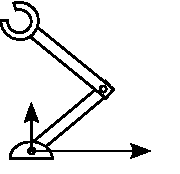
\includegraphics[width=0.27\textwidth]{figs/fwk2dofarm}
    % \def\svgwidth{0.4\textwidth}
    % \import{./figs/kinematics/}{fwk2dofarm.pdf_tex}
    \caption{Velocity (left) and force (right) manipulability ellipsoids for a 2 DoF planar arm ($n=m=2$). In this simple $2x2$ case, the ellipsoids collapse to simple ellipses. \td{add figure} }\label{fig:manipulability}
\end{figure}

\subsection{Manipulability Ellipsoid in Force space}

By virtue of the kineto-statics duality, similar considerations can be done in force space. In this case, we may want to consider a sphere in the space of joint torques:
\begin{equation}
\tau^T\cdot\tau = 1 \quad ,  \label{eq:forces:manipulability:torquesphere}
\end{equation}
which, thanks to \cref{eq:forces:statics}, is mapped into a \textsl{force manipulability ellipsoid}\index{Force Manipulability Ellipsoid}:
\begin{equation}
F^T \left[ J(q) \cdot J(q)^T \right] F = 1 \quad ,
\label{eq:forces:manipulability:forcemanipulability}
\end{equation}
This ellipsoid characterizes the forces at the end-effector that can be exerted by the robot on the environment in the given joint configuration $q$. It behaves similarly to the velocity manipulability ellipsoid, with one important difference: while the principal axes of both ellipsoids are in the same orientation, their magnitude is in inverse proportions.
As depicted in \cref{fig:manipulability} (right), the major axis in force space becomes the minor axis in velocity space and vice versa.
Therefore, a direction of high velocity manipulability corresponds to a direction of low force manipulability.

\subsection{Manipulability Considerations}

The velocity and force manipulability ellipsoids are useful for a variety of tasks, from identifying a suitable joint configuration to perform a specific task, to understand what it is possible for the robot to do in a specific configuration. Remember that, for a kinematically redundant manipulator (see \cref{sec:kinematics:diff:underover}), it is possible to be in the same task space configuration (e.g. end-effector pose) with multiple joint postures: therefore, a manipulability analysis may allow the robot designer to choose the configuration that better conforms to additional specifications (e.g. lower exerted force, lower energy consumption, better legibility of robot motion by humans, and more).

% \section{Force interactions and compliance}

% \section{Dynamics}\label{sec:forces:dynamics}


\section*{Take-home lessons}

\section*{Exercises}\small

\begin{enumerate}
\item Think about the four layers of abstraction we have just investigated (kinematics, differential kinematics, statics, dynamics).
\begin{enumerate}
\item Can you think of an application for which you would need a dynamic analysis? (Hint: this is generally something really hard)
\item What can be done by just looking at the static problem instead? (Hint: you are still considering an exchange of forces here)
\item What can you do with a robot from a purely kinematic perspective? (Hint: this is typically easy)
\end{enumerate}
\item Why are singular configuration dangerous for the robot and its surroundings? Think about the relationship between forces and velocities.
\item How can you ensure the robot ``stays away'' from singularities?
\item Program an application that displays the manipulability ellipsoids in force and velocity for a two-link planar arm (similar to \cref{fig:manipulability})---feel free to integrate this program with the kinematics exercise in \cref{chap:kinematics}. How does the manipulability ellipsoid relate to positional increments of the end-effector? What happens in a singularity? (Hint: the easiest singularity to find for robot manipulators is the ``stretched out'' configuration)
\item Use a robot simulator of your choice to access a robot manipulator with at least three DoFs in joint space that moves in 3D. How does the manipulability ellipsoid change in this case? (Hint: it is not an ellipse any more)
\item A manipulability analysis is purely geometrical and depends on joint configuration of a given kinematics. Therefore, it is possible to use this analysis to characterize other (non-traditional) robot ``arms'' as well. Think about a biomechanical analysis of the human arm: in which configurations you have maximum manipulability? Which configurations correspond to high exertion (i.e. high ``torques'') resulting in small exerted forces on the environment?
\end{enumerate}
